\documentclass[12pt]{article}
\usepackage{graphicx}
\usepackage{amsmath}
\usepackage{amsfonts}
\usepackage{hyperref}
\usepackage{geometry}
\geometry{a4paper}
\usepackage{booktabs}
\usepackage{float}
\usepackage{subcaption}
\usepackage{placeins}

\title{\textbf{Ortho-Vision}: Optimal therapeutic plan for implants}
\author{
    Rares Dan Tiago Goia, Group 923 \\ 
    Dragos Andrei Gavrus, Group 923 \\
    Babes-Bolyai University
}
\date{\today}

\begin{document}

\maketitle

\tableofcontents

\newpage

\begin{abstract}
This report documents the progress of the Ortho-Vision project, an AI-powered system designed for dental implant planning using segmentation models. The project aims to provide an optimal therapeutic plan for dental implants by leveraging deep learning techniques through segmentation and detection using dental imagery from radiographs.
\end{abstract}

\section{Introduction}
The Ortho-Vision project aims to assist dental implant planning by leveraging AI for accurate segmentation and detection of dental structures in radiographs. This system is designed to improve the planning process by providing clear and consistent implant guidance.

\section{Base Flow}
\subsection{Application Functionality}
The application is designed with functionalities that support end-to-end dental implant planning. It allows users to upload radiographs, segment dental features, and generate suggested implant plans based on segmented regions.

\subsection{Problem Description}
The goal of this project is to develop a solution for automatic segmentation of dental images, and detection of dental structures. This includes both a descriptive and formal problem analysis, aiming to create a reliable AI-based tool that can assist in identifying key dental regions necessary for implant placement.

\subsection{Related Work and Useful Tools and Technologies}
We explored existing dental segmentation models, including pre-trained options on Hugging Face, and reviewed literature on segmentation techniques commonly applied in medical imaging. Our toolkit includes TensorFlow, Keras and YOLO for model development, OpenCV and PIL for image processing, with additional experimentation using open-source pre-trained segmentation models to accelerate initial testing.

\section{Experimental Phase 1: Segmentation}
\subsection{Data Collection}
We collected a public dataset of multiple dental single-channel radiographs datasets from public sources with corresponding segmentation masks for key dental features. This had 1000 train images and 100 test images. The images have a resolution of 1615 x 840. These were normalized to 256 x 256.

\subsection{Methods and Algorithms}
We tested two primary models for segmentation:
\begin{itemize}
    \item \textbf{Pre-trained Dental Segmentator (Hugging Face):} A pre-trained model was initially tested, but results were suboptimal, likely due to dataset-specific variations. This model was tested on 100 2-dimensional radiographs and it was not trained on specific masks, as it should have already been trained specifically for dental segmentation.
    \item \textbf{U-Net Model:} Our U-Net model, from an existing deep-learning architecture, implemented with TensorFlow and Keras.
    \begin{itemize}
        \item \textbf{Experiment 1:} Used a partition of 500 images from the public dataset for training with a batch size of 8 and 50 epochs, achieving an accuracy of approximately 92\% on the validation set. 
        \item \textbf{Experiment 2:} Used the whole public dataset for training with a batch size of 32 and 30 epochs, yielding slightly higher accuracy at 94.5\% on the validation set, indicating that the larger batch size and longer training improved the model's performance.
    \end{itemize}
    The best results were achieved in Experiment 2, where the combination of a larger batch size and additional training epochs allowed the model to converge more effectively.
\begin{figure}
    \centering
    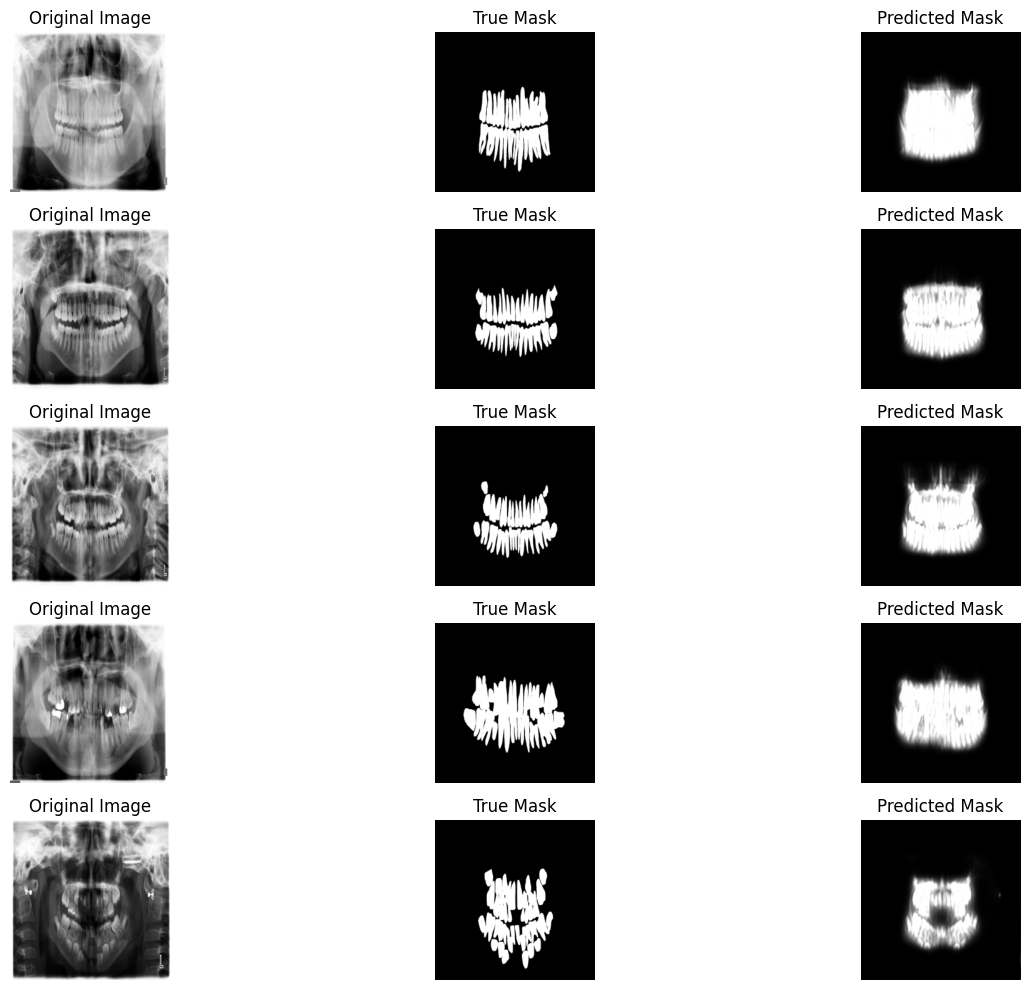
\includegraphics[width=0.5\linewidth]{output.png}
    \caption{Results from our first experiment of U-Net segmentation model showing accurate predicted masks of dental features.}
    \label{fig:enter-label}
\end{figure}
\begin{figure}[H]
    \centering
    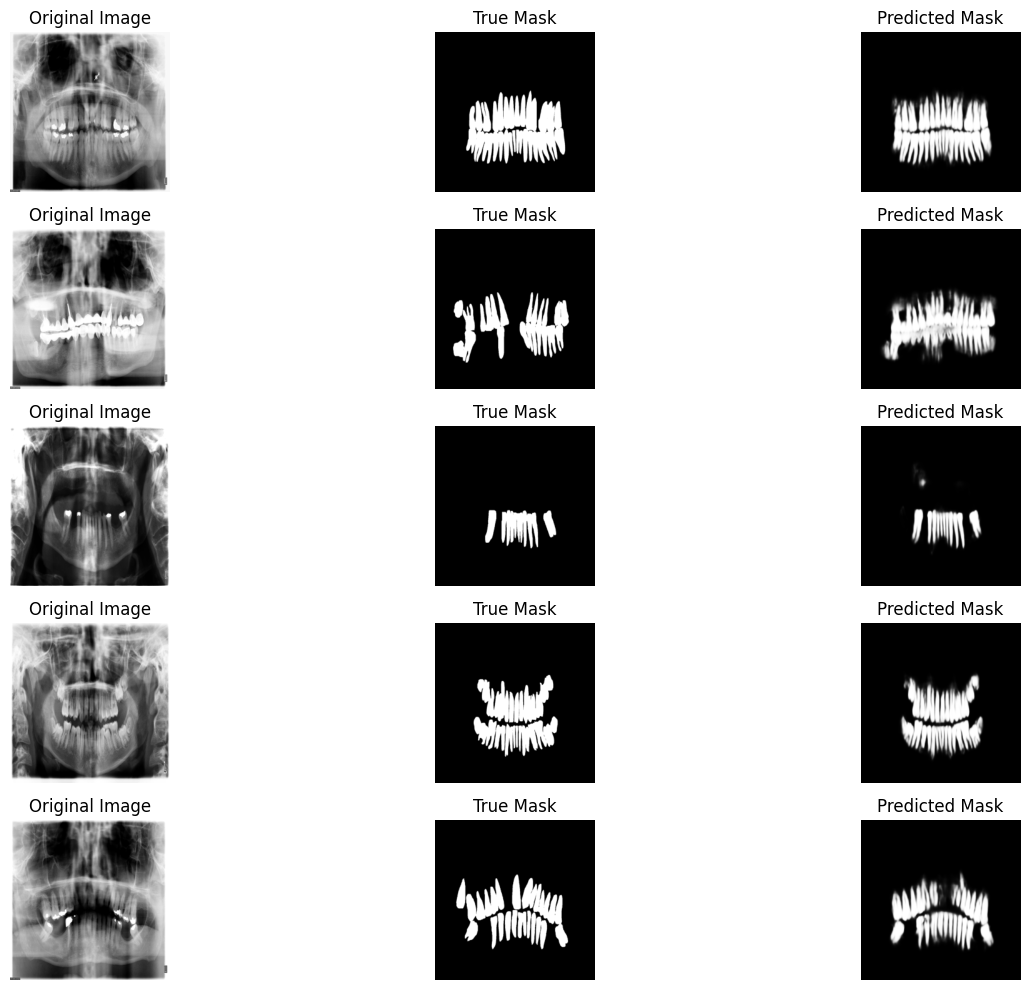
\includegraphics[width=0.5\linewidth]{theeth_v2.png}
    \caption{Results from our second experiment of U-Net segmentation model showing accurate predicted masks of dental features.}
    \label{fig:enter-label}
\end{figure}
\end{itemize}

\subsection{Results and Discussion}
The U-Net model significantly outperformed the pre-trained Dental Segmentator, especially with the second experiment, achieving accurate and reliable segmentations on our dataset. This model is expected to be central to the overall implant planning application, given its robust performance.

\begin{figure}[htbp]
    \centering
    \begin{subfigure}[b]{0.45\textwidth}
        \centering
        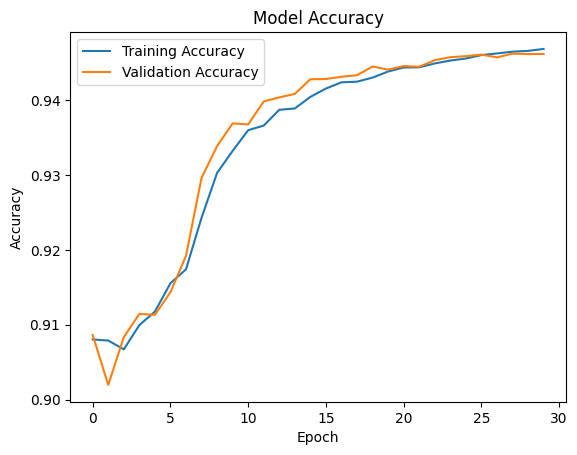
\includegraphics[width=\textwidth]{unet_accuracy.png}
        \caption{Accuracy Convergence}
        \label{fig:image1}
    \end{subfigure}
    \hfill
    \begin{subfigure}[b]{0.45\textwidth}
        \centering
        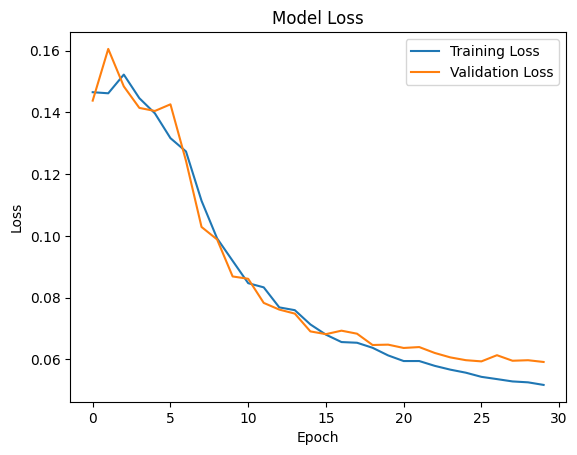
\includegraphics[width=\textwidth]{unet_loss.png}
        \caption{Loss Convergence}
        \label{fig:image2}
    \end{subfigure}
    \caption{Metrics for best performing U-Net}
    \label{fig:side_by_side}
\end{figure}

\section{Experimental Phase 2: Object Detection - Anomalies Identification}

\subsection{Data Collection}
In this phase, we received proprietary data from UMF University, provided through collaboration with Prof. Mihaela Hedeșiu. The dataset contains 1000 images for training, 100 for validation, and 100 for testing. The images have a resolution of 2775x1475. It contains 12 classes: 'IMP', 'PRR', 'OBT', 'END', 'CAR', 'BON', 'IMT', 'API', 'ROT', 'FUR', 'APS', 'ROR', 'ORD', 'SRD'.  Using this dataset, we trained a YOLOv11 model to detect dental structures and extract key characteristics for each tooth. This approach complements the segmentation task by adding object detection capabilities, providing a comprehensive analysis of dental features.

\subsection{Methods and Algorithms}
We utilized the YOLOv11 model for its state-of-the-art performance in object detection tasks. This model was pre-trained on COCO dataset. The model was trained on the proprietary dataset with the following configuration:
\begin{itemize}
    \item \textbf{Training Configuration:} Default configuration from Ultralyitcs library. Trained on the whole recieved dataset.
    \item \textbf{Model Objective:} To detect dental structures and annotate key characteristics for each tooth, such as previous work done by the dentists.
    \begin{figure}[H]
    \centering
    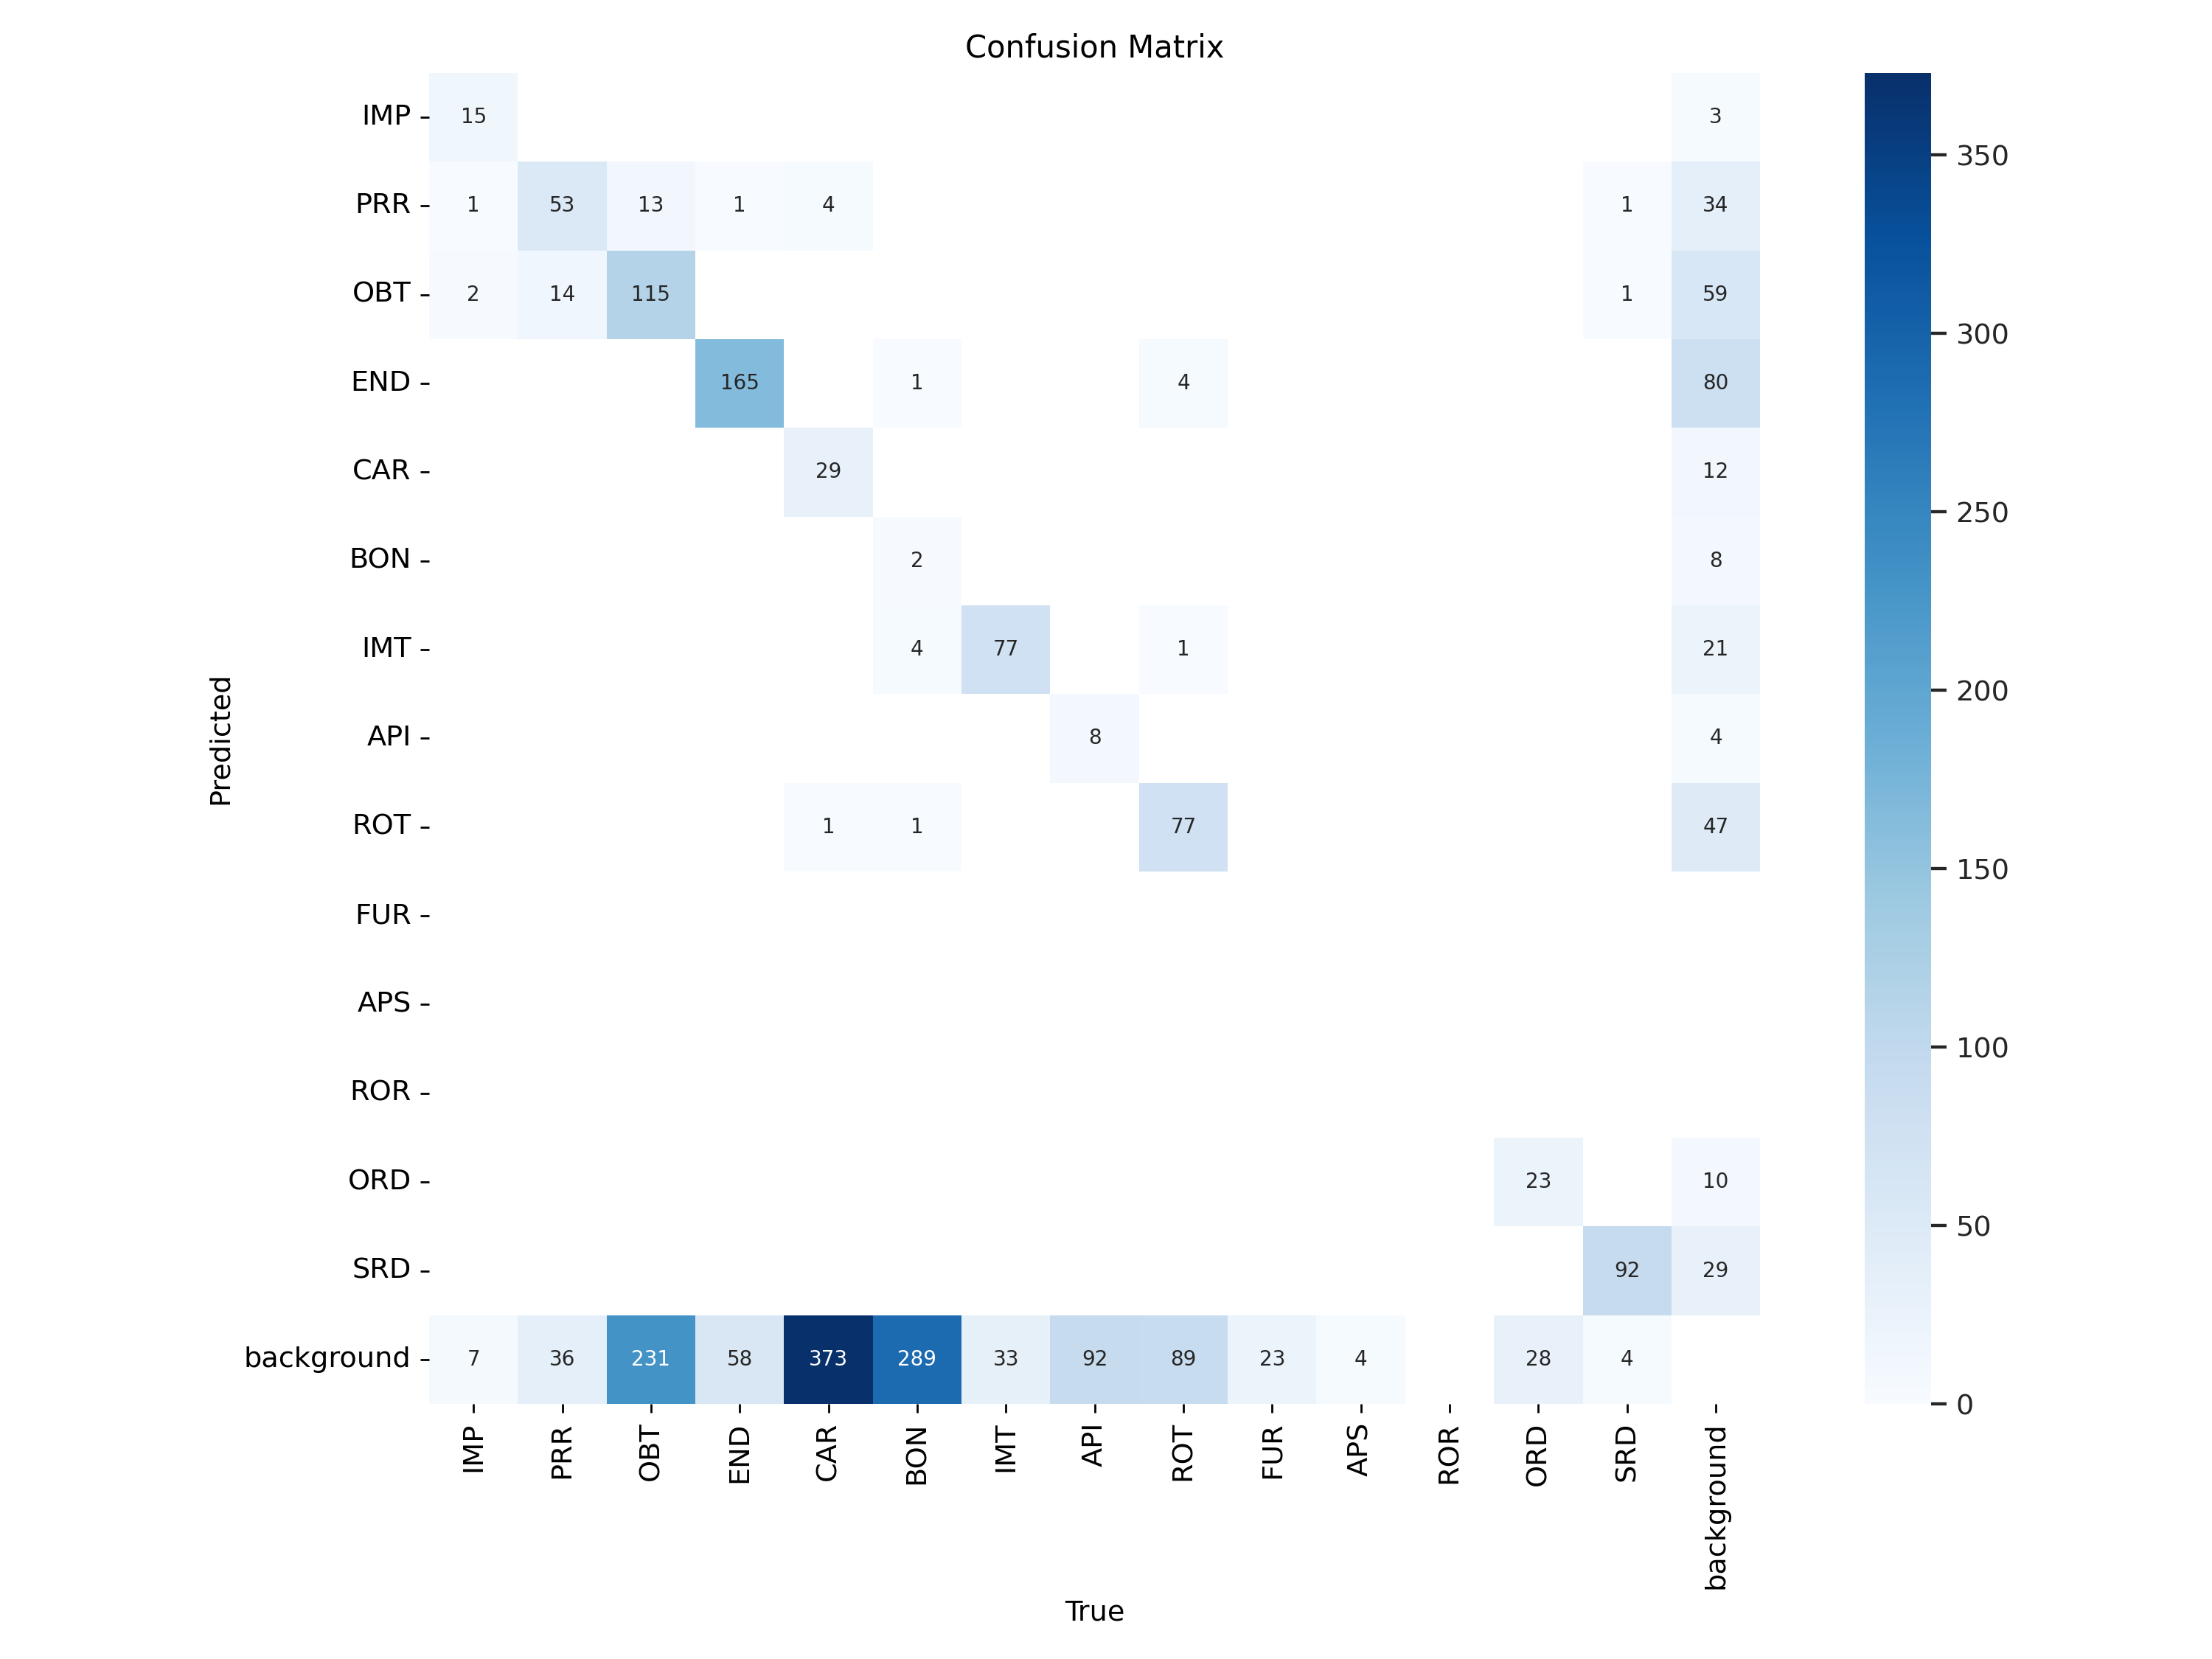
\includegraphics[width=0.6\linewidth]{yolo_conf_matrix_1.png}
    \caption{Confusion Matrix from YOLOv11 detection for each annotaion class.}
    \label{fig:yolo-output}
\end{figure}
\end{itemize}

\subsection{Results and Discussion}
The YOLOv11 model Successfully identified individual teeth and their attributes, providing valuable insights for dental implant planning.

\begin{table}[htbp]
    \centering
    \caption{Detection Metrics for Classes}
    \begin{tabular}{lrrrrrr}
        \toprule
        \textbf{Class} & \textbf{Images} & \textbf{Instances} & \textbf{Box(P)} & \textbf{R} & \textbf{mAP50} & \textbf{mAP50-95} \\
        \midrule
        all  & 153  & 1972 & 0.549 & 0.386  & 0.369  & 0.167 \\
        IMP  & 10   & 25   & 0.713 & 0.595  & 0.632  & 0.342 \\
        PRR  & 49   & 103  & 0.477 & 0.592  & 0.467  & 0.240 \\
        OBT  & 80   & 359  & 0.539 & 0.401  & 0.413  & 0.135 \\
        END  & 79   & 224  & 0.655 & 0.747  & 0.679  & 0.269 \\
        CAR  & 108  & 407  & 0.617 & 0.0688 & 0.124  & 0.0364 \\
        BON  & 49   & 297  & 0.200 & 0.0168 & 0.0332 & 0.00999 \\
        IMT  & 46   & 110  & 0.666 & 0.652  & 0.600  & 0.299 \\
        API  & 45   & 100  & 0.486 & 0.060  & 0.121  & 0.0391 \\
        ROT  & 43   & 171  & 0.457 & 0.474  & 0.397  & 0.136 \\
        FUR  & 15   & 23   & 1.000 & 0.000  & 0.0142 & 0.00403 \\
        APS  & 1    & 4    & 0.000 & 0.000  & 0.000  & 0.000 \\
        ORD  & 18   & 51   & 0.646 & 0.471  & 0.404  & 0.200 \\
        SRD  & 20   & 98   & 0.682 & 0.939  & 0.916  & 0.466 \\
        \bottomrule
    \end{tabular}
    \label{tab:detection_metrics}
\end{table}

\begin{figure}[H]
    \centering
    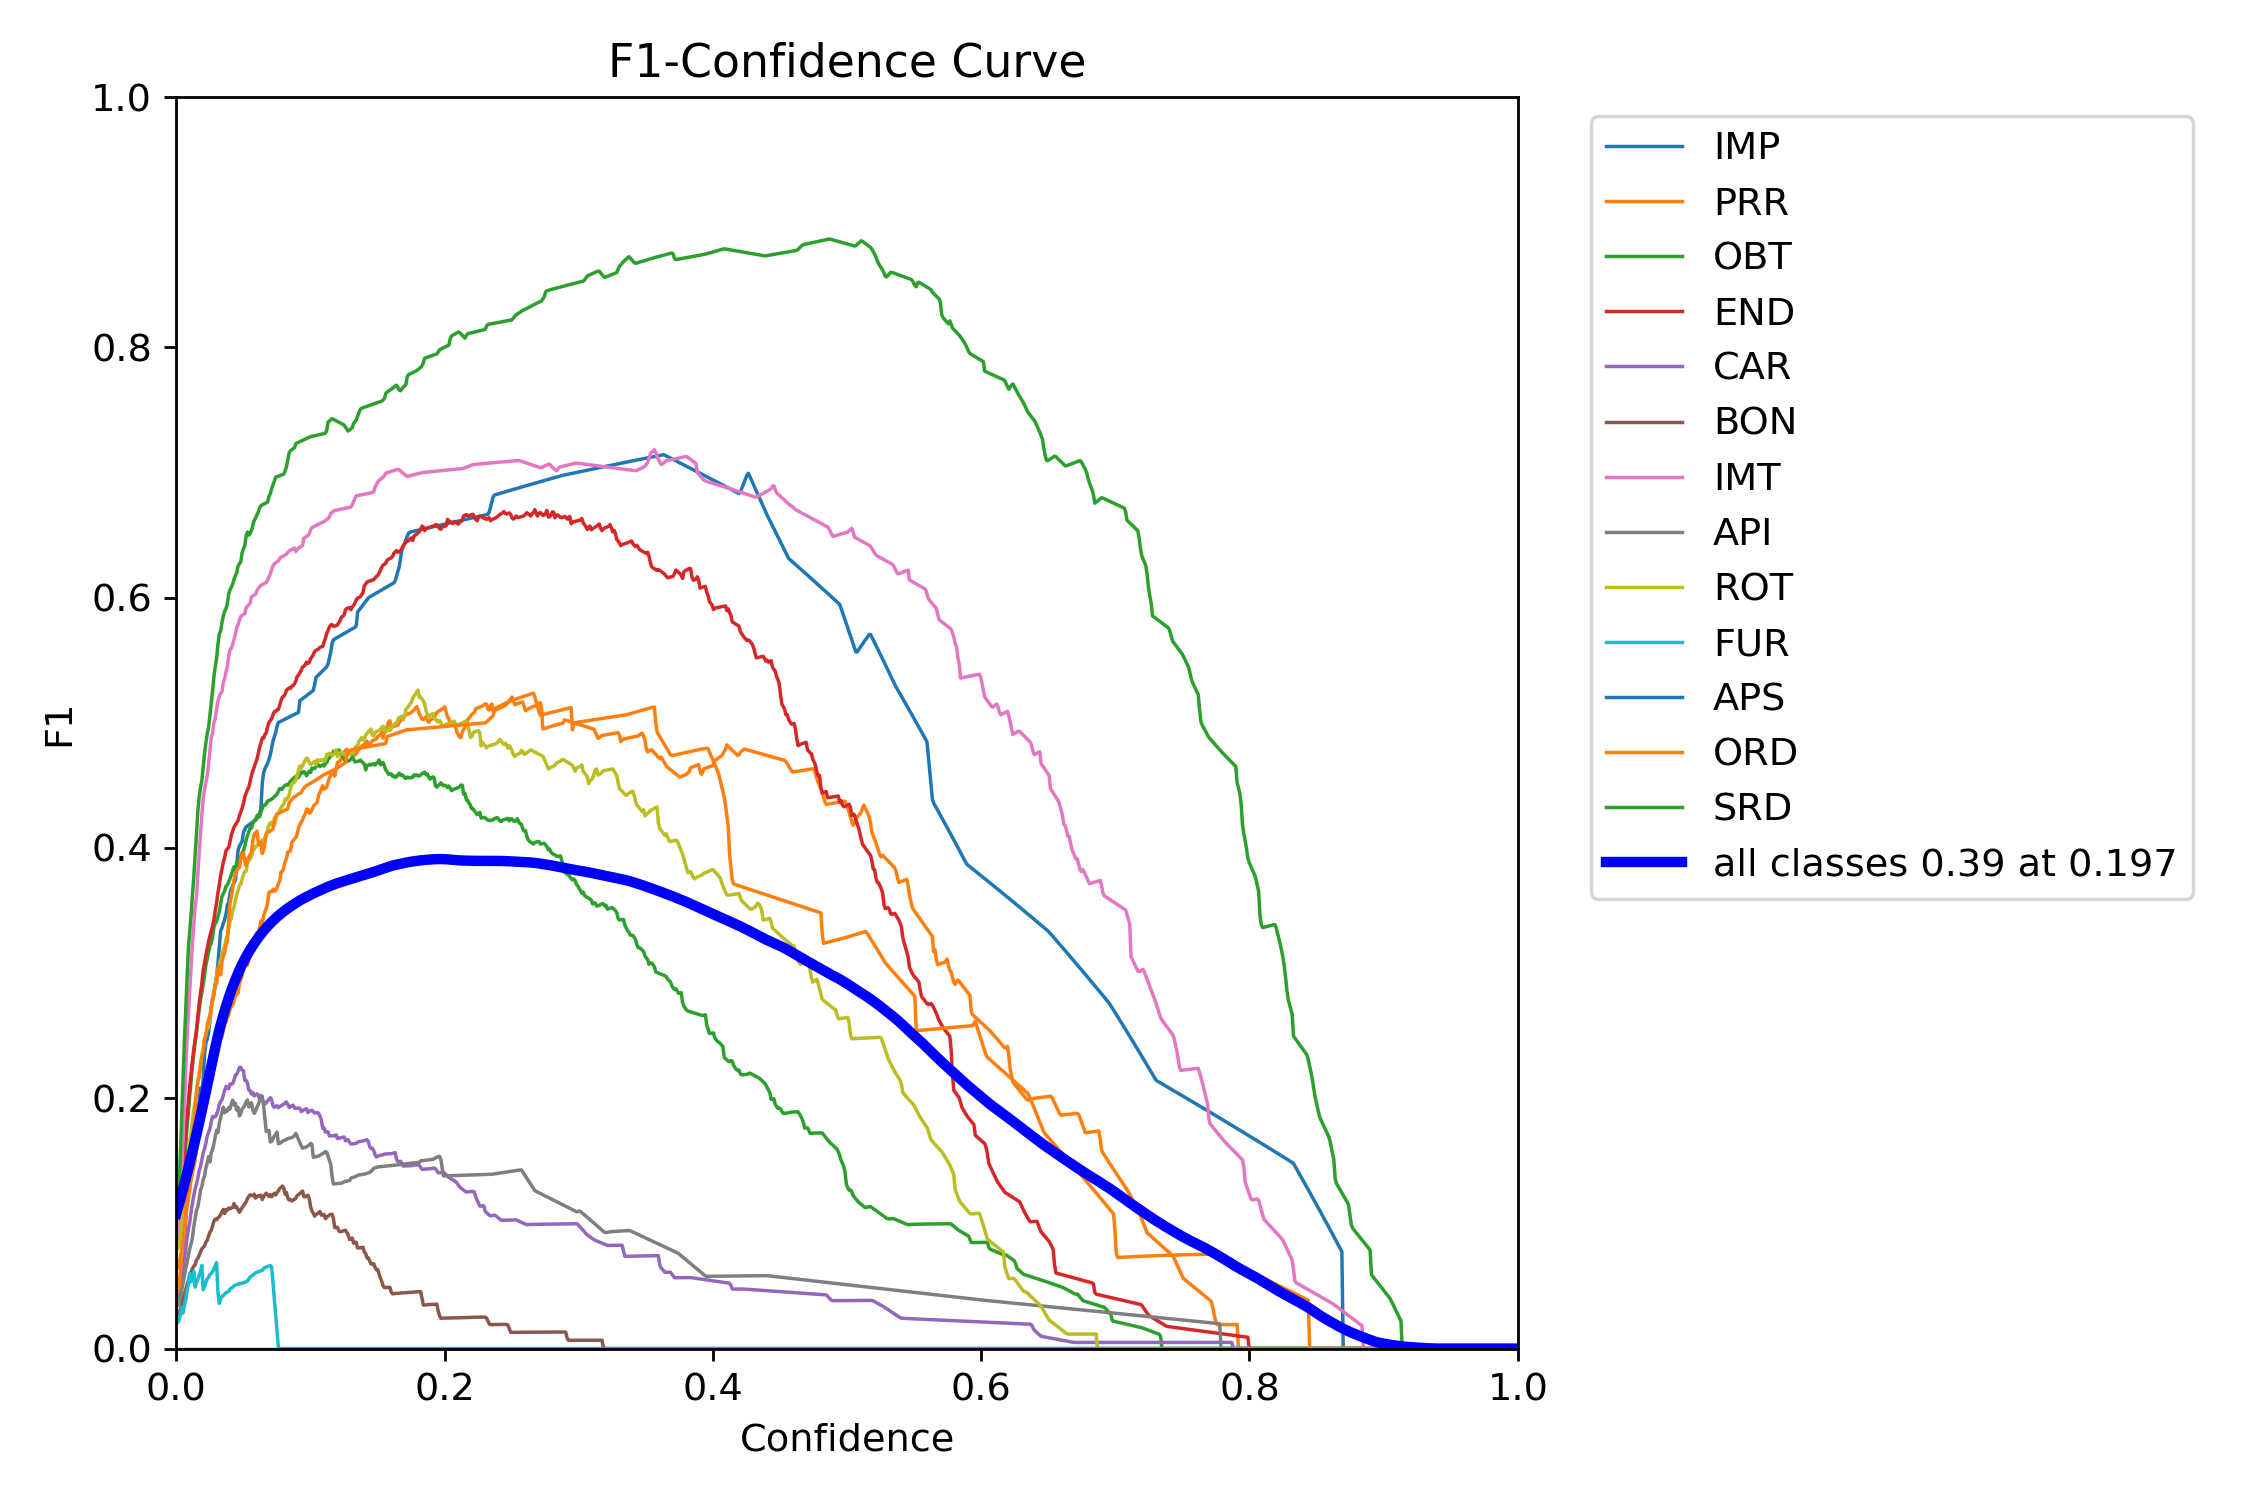
\includegraphics[width=0.6\linewidth]{F1_curve_1.png}
    \caption{Validation F1 score.}
    \label{fig:yolo-output}
\end{figure}

\newpage

The results indicate that YOLOv11 is an effective tool for detecting dental structures and extracting detailed characteristics. This capability will be integrated into the final application to enhance the planning process by combining segmentation with object detection.

\begin{figure}[H]
    \centering
    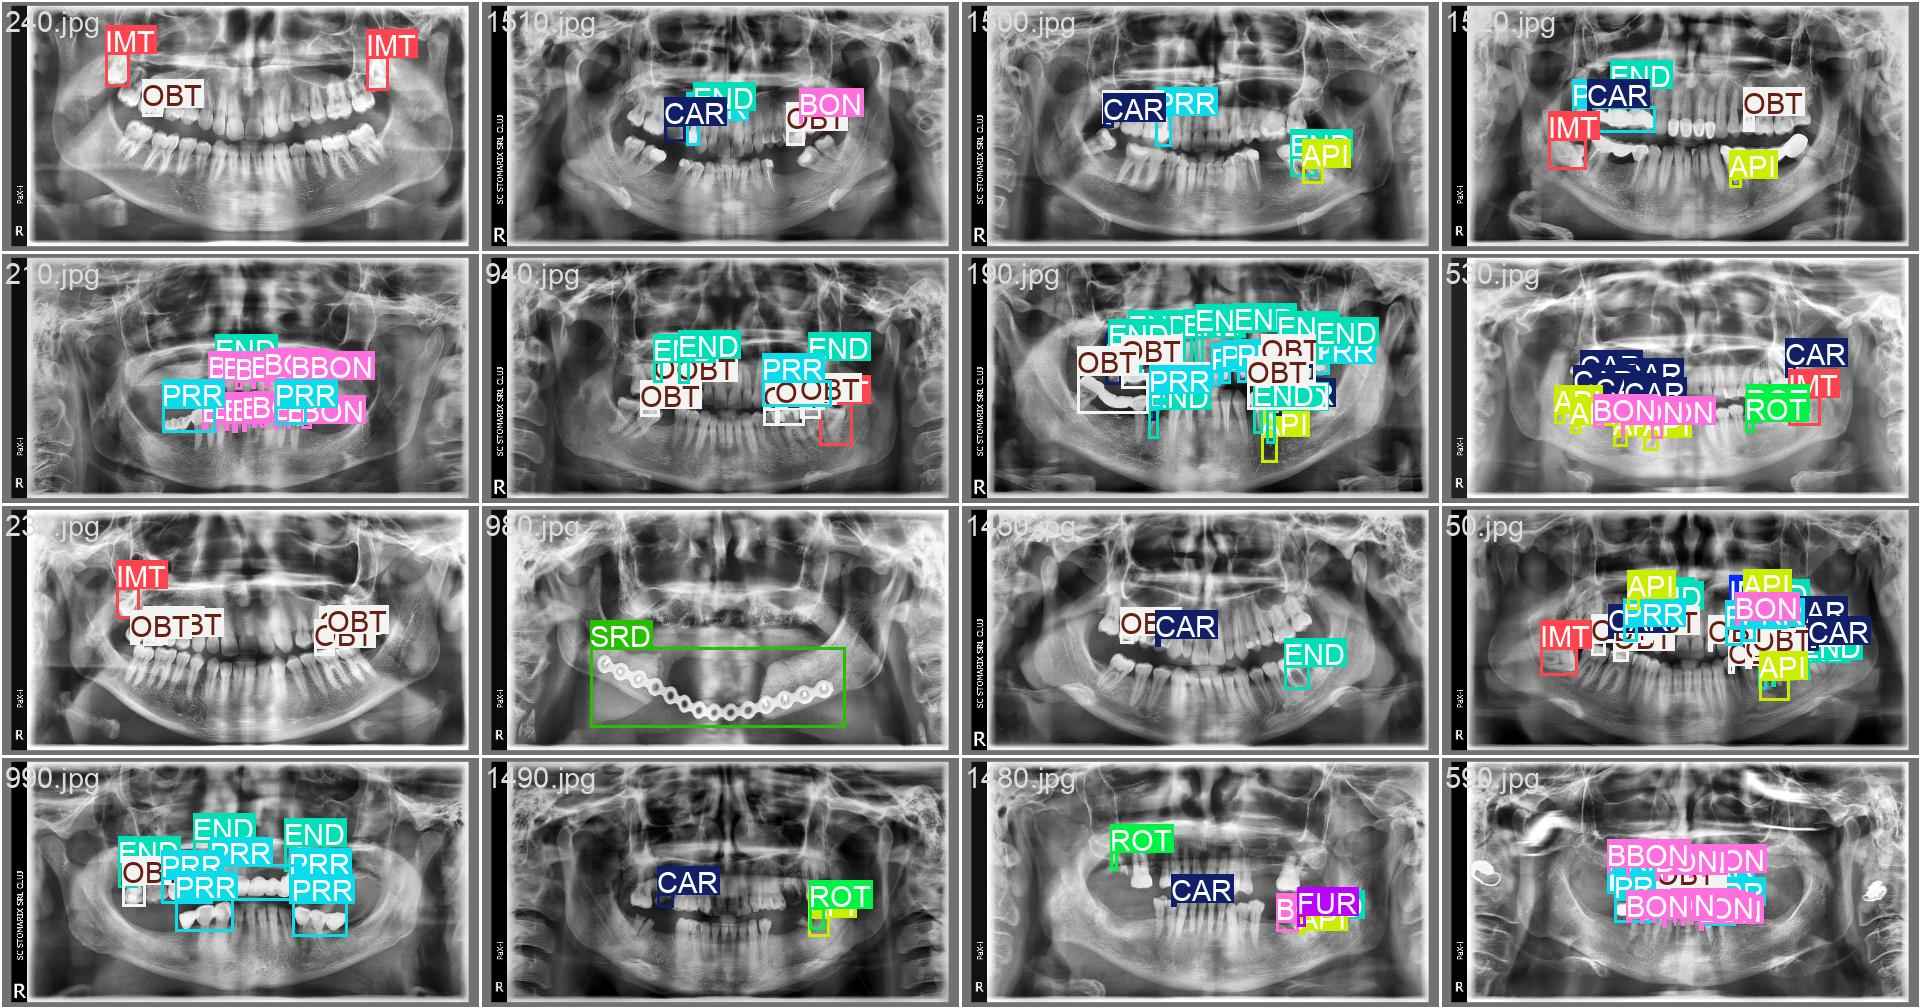
\includegraphics[width=0.6\linewidth]{val_batch1_labels.jpg}
    \caption{Results from YOLOv11 detection, highlighting dental structures and annotations for each tooth.}
    \label{fig:yolo-output}
\end{figure}

\newpage

\section{Experimental Phase 3: Object Detection - Teeth Identification}

\subsection{Data Collection}
In this phase, we received more proprietary data from UMF University, provided through collaboration with Prof. Mihaela Hedeșiu. The dataset contains 1000 images for training and 100 for validation/testing. The images have a resolution of 2775x1475. It contains 32 classes each representing an individual tooth. Using this dataset, we trained another YOLOv11 model to detect each individual tooth to be able to match each tooth with its corresponding anomaly. This approach complements the previous object detection task, providing more accurate details about each radiograph.

\subsection{Methods and Algorithms}
We utilized the YOLOv11 model for its state-of-the-art performance in object detection tasks. This model was pre-trained on COCO dataset. The model was trained on the proprietary dataset with the following configuration:
\begin{itemize}
    \item \textbf{Training Configuration:} Default configuration from Ultralyitcs library. Trained on the whole recieved dataset.
    \item \textbf{Model Objective:} To detect each individual teeth in the dental structures.
    \begin{figure}[H]
    \centering
    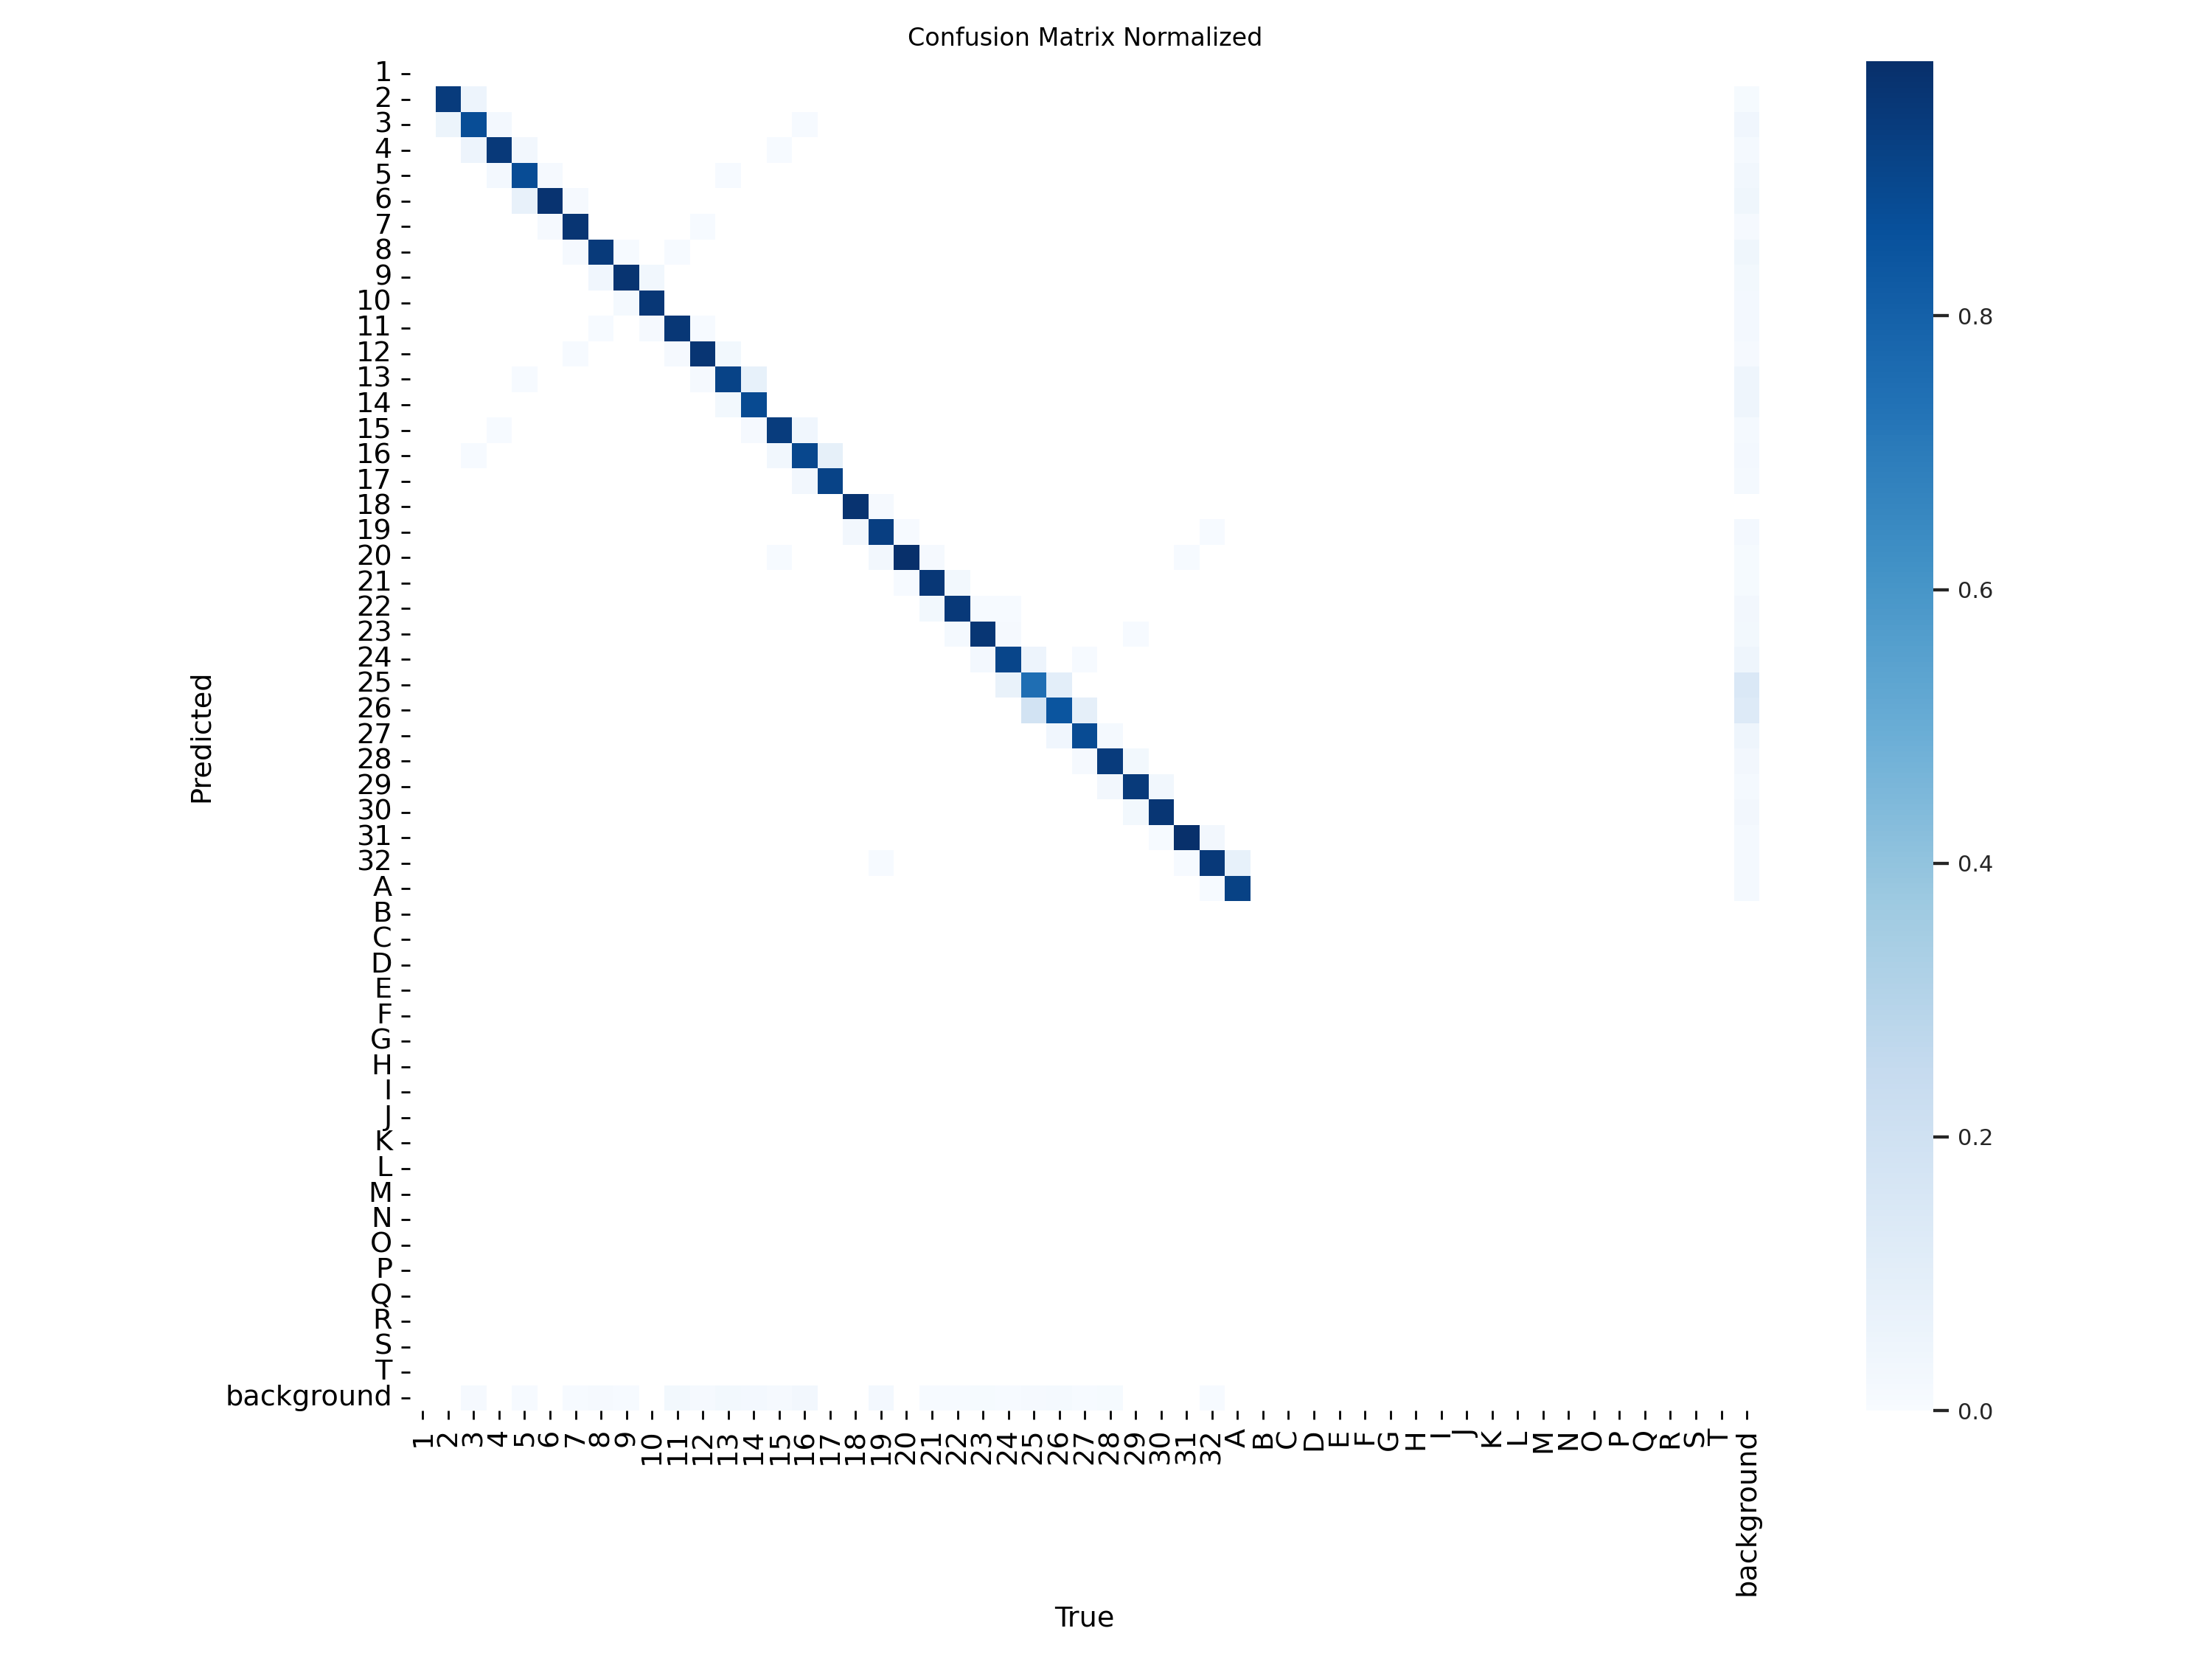
\includegraphics[width=0.6\linewidth]{confusion_matrix_normalized.png}
    \caption{Confusion Matrix from YOLOv11 detection for each annotaion class.}
    \label{fig:yolo-output}
\end{figure}
\end{itemize}

\subsection{Results and Discussion}
The YOLOv11 model Successfully identified individual teeth and their attributes, providing valuable insights for dental implant planning.

\begin{table}[htpb]
    \centering
    \caption{Detection Metrics for All Teeth Classes}
    \begin{tabular}{lrrrrrrr}
        \toprule
        \textbf{Class} & \textbf{Images} & \textbf{Instances} & \textbf{Box(P)} & \textbf{R} & \textbf{mAP50} & \textbf{mAP50-95} \\
        \midrule
        all & 183 & 4635 & 0.949 & 0.939 & 0.975 & 0.701 \\
        2 & 70 & 70 & 0.942 & 0.926 & 0.967 & 0.658 \\
        3 & 139 & 139 & 0.955 & 0.911 & 0.957 & 0.730 \\
        4 & 141 & 141 & 0.934 & 0.957 & 0.959 & 0.706 \\
        5 & 143 & 143 & 0.929 & 0.895 & 0.951 & 0.674 \\
        6 & 144 & 144 & 0.932 & 0.951 & 0.963 & 0.654 \\
        7 & 165 & 165 & 0.976 & 0.967 & 0.990 & 0.694 \\
        8 & 162 & 162 & 0.987 & 0.939 & 0.987 & 0.666 \\
        9 & 161 & 161 & 0.963 & 0.969 & 0.988 & 0.696 \\
        10 & 162 & 162 & 0.990 & 0.944 & 0.993 & 0.691 \\
        11 & 162 & 162 & 0.961 & 0.921 & 0.982 & 0.656 \\
        12 & 164 & 164 & 0.945 & 0.936 & 0.973 & 0.689 \\
        13 & 156 & 156 & 0.921 & 0.903 & 0.948 & 0.622 \\
        14 & 142 & 142 & 0.961 & 0.901 & 0.980 & 0.689 \\
        15 & 145 & 145 & 0.950 & 0.924 & 0.966 & 0.719 \\
        16 & 138 & 138 & 0.911 & 0.894 & 0.961 & 0.734 \\
        17 & 69 & 69 & 0.884 & 0.928 & 0.974 & 0.717 \\
        18 & 74 & 74 & 0.973 & 0.977 & 0.992 & 0.766 \\
        19 & 142 & 142 & 0.959 & 0.951 & 0.988 & 0.815 \\
        20 & 135 & 135 & 0.940 & 0.978 & 0.988 & 0.833 \\
        21 & 161 & 161 & 0.974 & 0.940 & 0.980 & 0.730 \\
        22 & 160 & 160 & 0.963 & 0.972 & 0.989 & 0.716 \\
        23 & 175 & 175 & 0.966 & 0.960 & 0.991 & 0.701 \\
        24 & 170 & 170 & 0.947 & 0.929 & 0.978 & 0.647 \\
        25 & 172 & 172 & 0.917 & 0.896 & 0.947 & 0.590 \\
        26 & 170 & 170 & 0.887 & 0.882 & 0.946 & 0.588 \\
        27 & 166 & 166 & 0.963 & 0.945 & 0.970 & 0.618 \\
        28 & 174 & 174 & 0.965 & 0.960 & 0.981 & 0.688 \\
        29 & 167 & 167 & 0.945 & 0.932 & 0.975 & 0.712 \\
        30 & 148 & 148 & 0.946 & 0.947 & 0.975 & 0.680 \\
        31 & 145 & 145 & 0.934 & 0.977 & 0.983 & 0.798 \\
        32 & 138 & 138 & 0.946 & 0.964 & 0.990 & 0.802 \\
        \bottomrule
    \end{tabular}
    \label{tab:teeth_detection_metrics_phase2}
\end{table}


\begin{figure}[H]
    \centering
    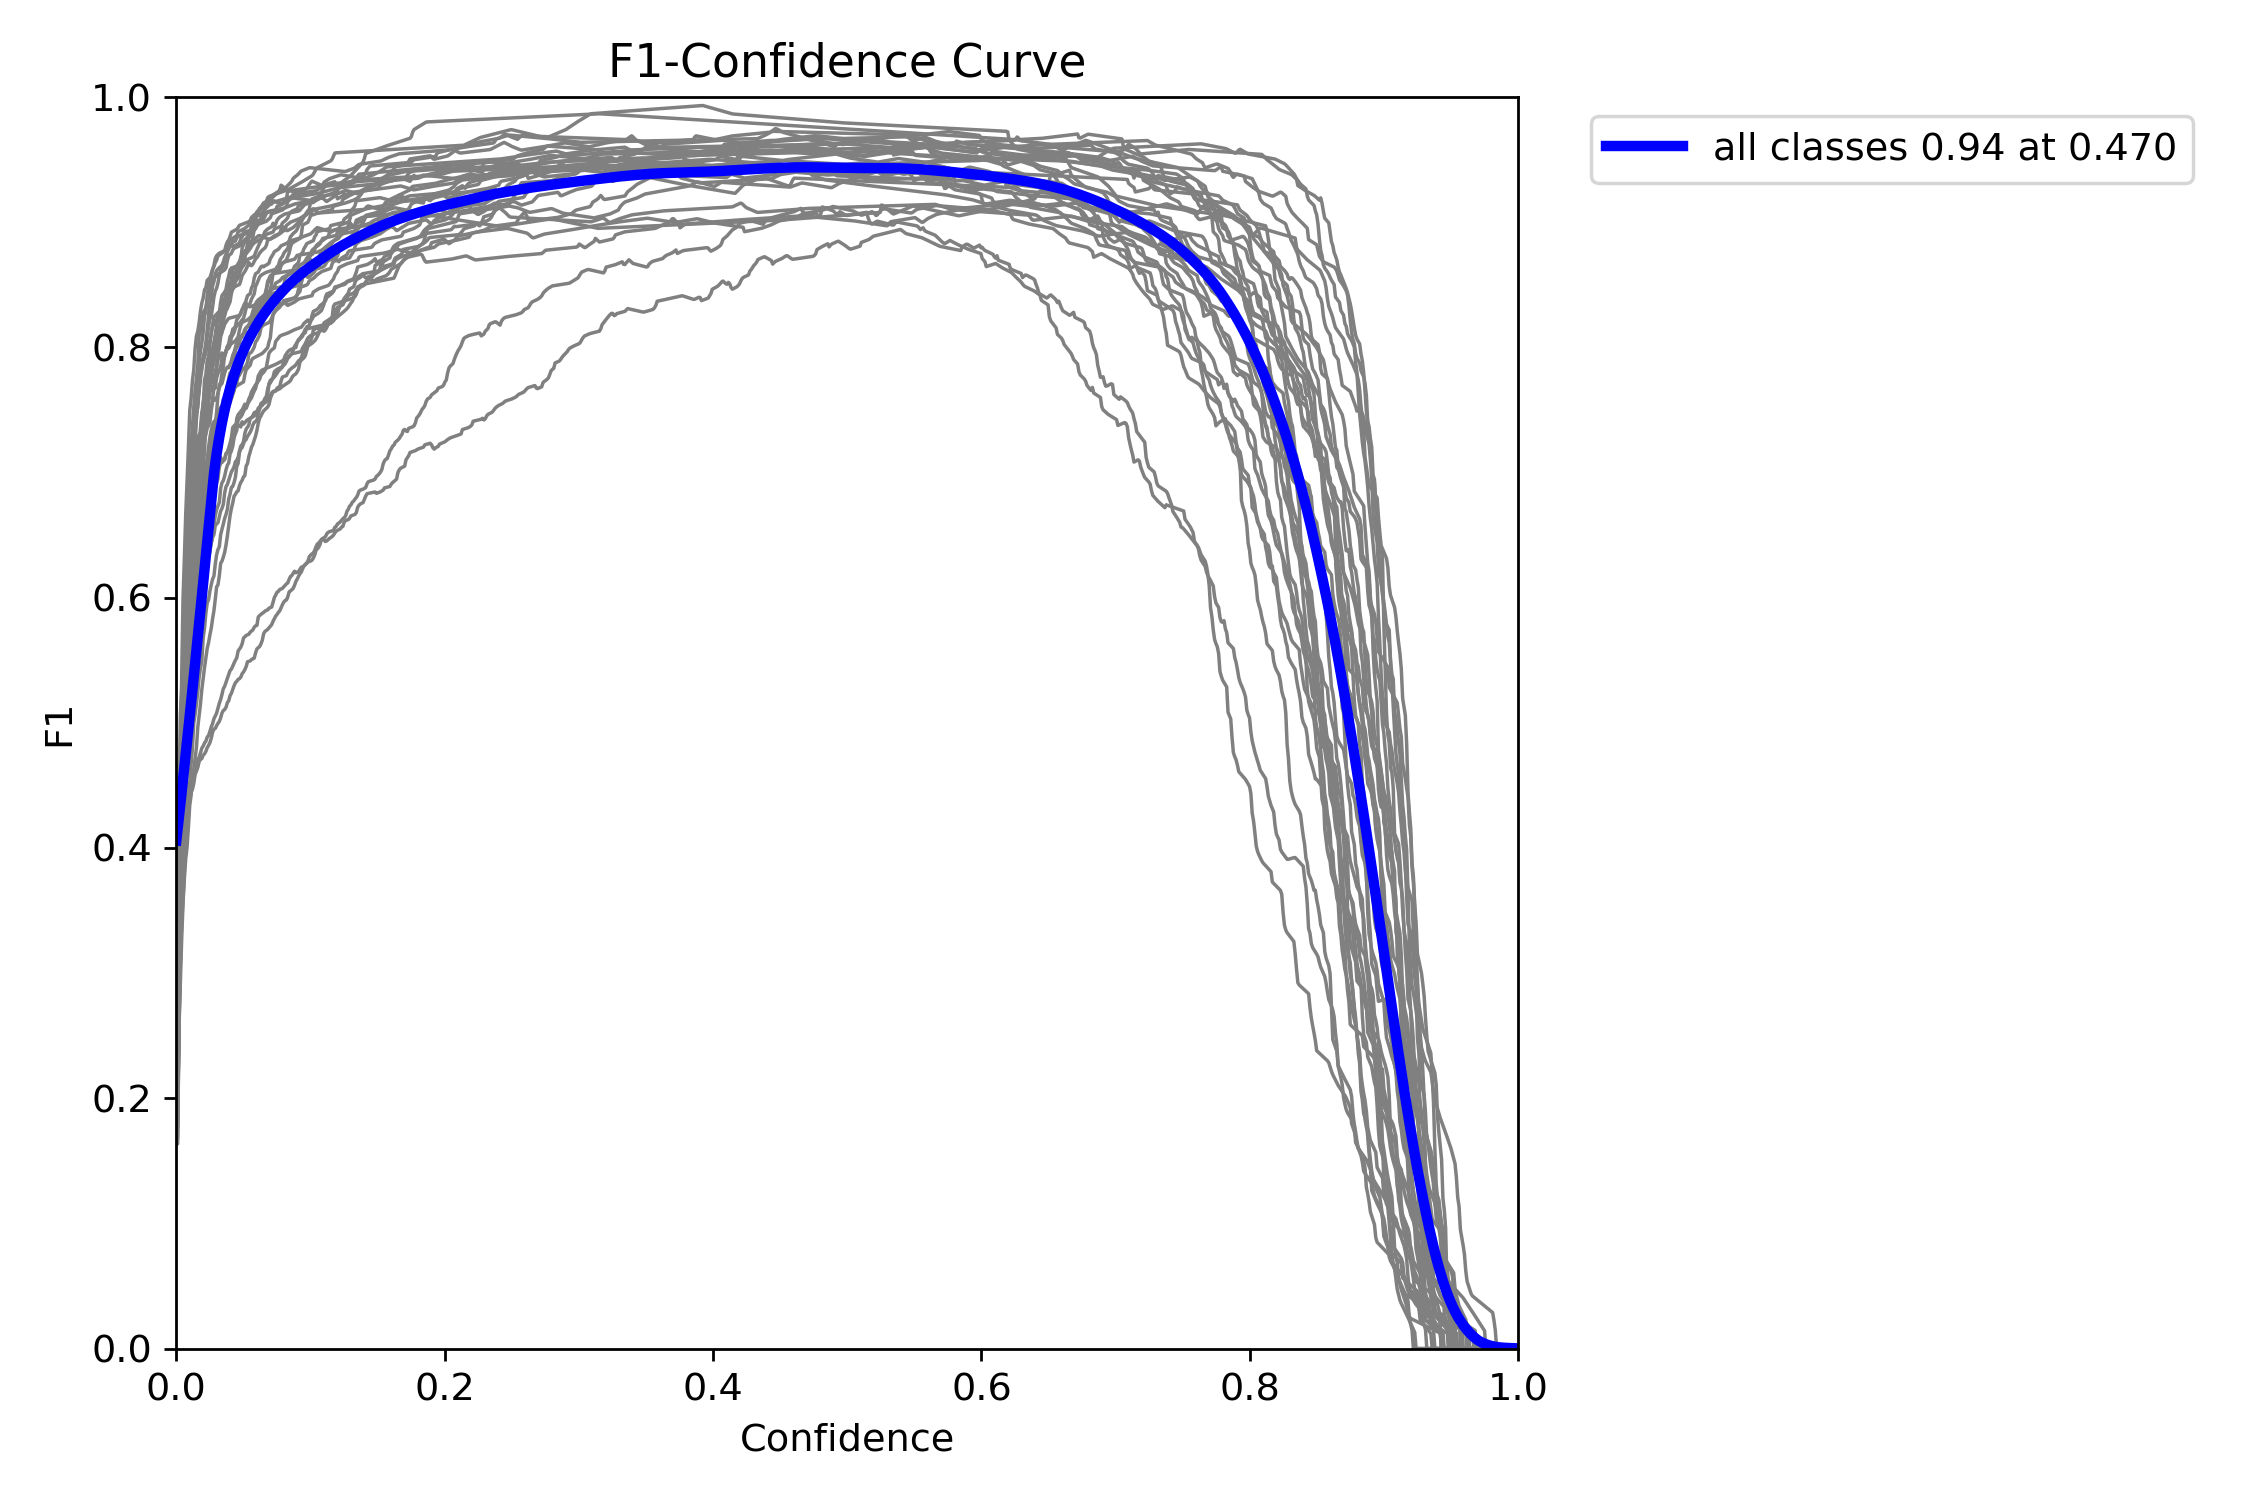
\includegraphics[width=0.6\linewidth]{F1_curve.png}
    \caption{Validation F1 score.}
    \label{fig:yolo-output}
\end{figure}

\newpage

The results indicate that YOLOv11 is an effective tool for detecting individual teeth in dental structures. This capability will be integrated into the final application to enhance the planning process by combining the two object detection models.

\begin{figure}[H]
    \centering
    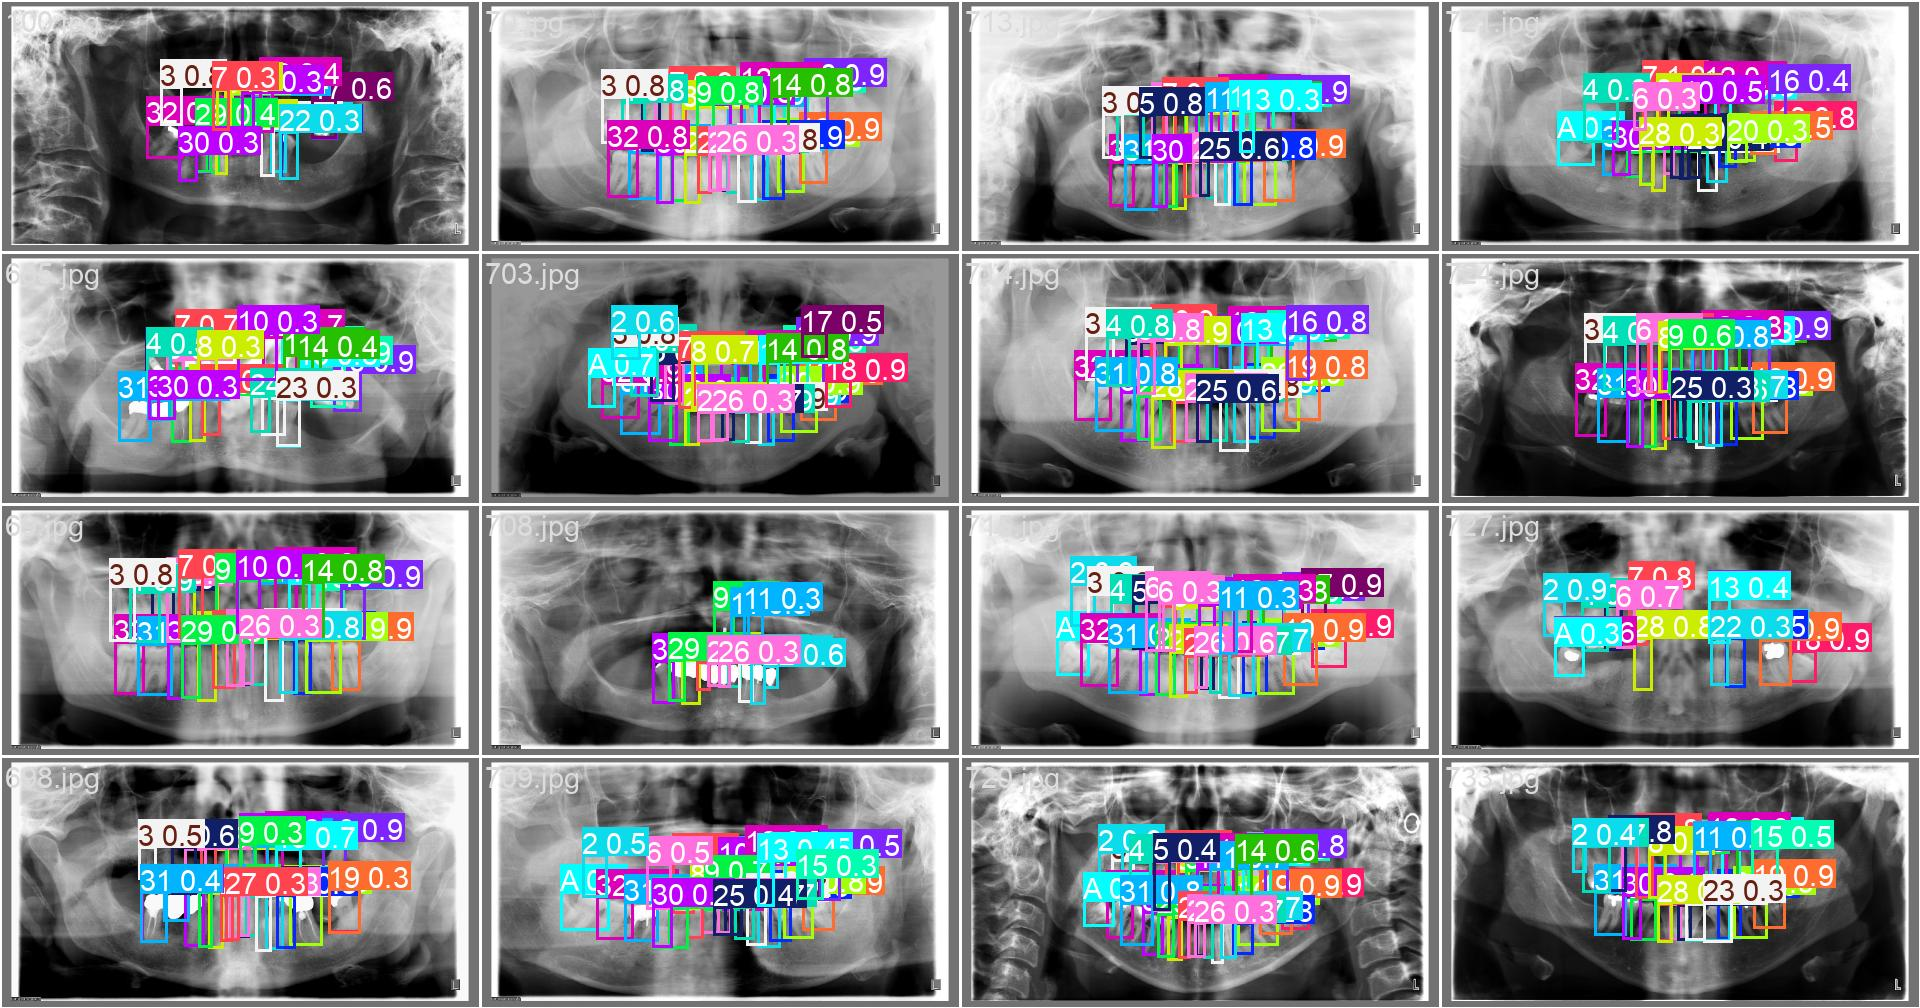
\includegraphics[width=0.6\linewidth]{val_batch0_pred.jpg}
    \caption{Results from YOLOv11 detection, highlighting individual teeth in dental structures and annotations for each tooth.}
    \label{fig:yolo-output}
\end{figure}

\newpage

\section{Experimental Phase 4: Model Improvements and Pipeline}
This phase will focus on further optimizing our winning models model, introducing additional data preprocessing steps, and experimenting with ensemble methods or advanced architectures to improve accuracy further.

\subsection{Results and Discussion}
We expect that these improvements will lead to higher accuracy and more reliable segmentation and detection outputs, particularly in complex or noisy images. Results from these experiments will be detailed as they are completed.

\section{Future Work}
Future improvements will focus on integrating post-processing techniques for refinement of segmentation, expanding the dataset with 3-dimensional radiographs, and evaluating additional model architectures. We also aim to implement the system as a complete dental implant planning tool with a user-friendly interface and easy-to-interpret outputs.

\end{document}


